% !TEX program = xelatex
\documentclass[11pt,a4paper]{article}
\usepackage[a4paper,margin=2.2cm]{geometry}
\usepackage{xeCJK}
\setCJKmainfont[BoldFont={Source Han Serif TW Bold},ItalicFont={Source Han Serif TW Light}]{Source Han Serif TW}
\setCJKsansfont[BoldFont={Source Han Serif TW Bold}]{Source Han Serif TW Regular}
\setmainfont{Times New Roman}
\usepackage{amsmath,amssymb}
\usepackage{graphicx}
\usepackage{booktabs}
\usepackage{caption}
\usepackage[hidelinks]{hyperref}
\usepackage{array}
\usepackage{algorithm}
\usepackage{algpseudocode}
\usepackage{enumitem}
\usepackage{xcolor}
\usepackage{titlesec}
\titleformat*{\section}{\large\bfseries}
\titleformat*{\subsection}{\normalsize\bfseries}
\setlength{\parskip}{2pt}
\setlength{\itemsep}{0pt}
\renewcommand{\baselinestretch}{1.05}
\captionsetup{font=small,skip=4pt}

\title{\vspace{-1.2cm}\textbf{便利商店個人化餐食推薦之最佳化模型}\\[2pt]
\large 以 MILP 與 GRASP-LS 啟發式並用之決策架構}
\author{Group 13\;|\;B13705005 宋宇倫、B13705011 陳芃慈、B13705020 陳鼎元、B13705029 蔡冠毅\\
Department of Information Management, National Taiwan University}
\date{June 6, 2026}

\begin{document}
\maketitle
\vspace{-0.5cm}

\section{Introduction}
便利商店是台灣大學生與上班族最高頻次的即時餐食取得管道：門市密度高、購買快速、商品標示完整。然而消費者在挑選時同時面臨成本、熱量、蛋白質、糖、鈉與飽足感等多重考量。若僅以「最低價」為依據，容易選到高糖高鈉商品；若僅追求「健康」，又可能讓單餐花費過高。實務上，便利商店亦頻繁推出「飯糰＋飲料」、「麵食＋蛋」等捆綁優惠，使得最終的支付成本依賴於是否使用組合，而非單品原價之直接加總。

本研究將上述決策抽象為一個含優惠組合、含個人化營養限制與含歷史多樣性懲罰的混合整數線性規劃（MILP）。決策者為使用者本人，其在指定情境模式（輕食／正餐／宵夜型）、基本生理資訊（性別、年齡、身高、體重）、活動量與健康目標（維持／減脂／增肌）後，模型應自動推薦一組符合預算與營養底線、且具備多樣性的單餐組合。決策的核心 trade-off 為：
\begin{itemize}[leftmargin=*]
\item 成本最小化 vs.\ 蛋白質最大化（高蛋白食物通常較貴）。
\item 嚴格遵守營養區間 vs.\ 可行解之存在性（過嚴限制易導致無解）。
\item 短期內推薦多樣性 vs.\ 客觀「最佳」商品的反覆勝出。
\end{itemize}
為兼顧上述目標，本研究於目標函數中加入軟性懲罰項，並引入歷史權重 $h_i$ 控制多樣性。此外，由於 MILP 在大型商品集（數百項）下的求解時間可能過長，本研究另自行設計一啟發式 \textbf{GRASP-LS}（Greedy Randomized Adaptive Search Procedure + Local Search），可在毫秒到秒級時間內回傳可行且近似最優的解，並以 Gurobi 為基準量化最佳化差距。

\section{Problem Description}
考慮一位使用者欲在便利商店購買一餐。給定商品集合與其價格、營養標示，以及一組「雙品項／三品項優惠組合」，使用者輸入情境模式、生理資訊、健康目標與預算上限後，系統需決定：
\begin{enumerate}[leftmargin=*,nosep]
\item 哪些商品以原價單品方式被選入；
\item 哪些優惠組合應被啟用（將其包含的商品一併納入推薦）；
\item 在預算與營養條件互相衝突時，應允許哪些限制以最小代價稍微鬆弛。
\end{enumerate}

模型輸出為一份單餐推薦清單與其總熱量、蛋白質、脂肪、碳水、糖、鈉等含量。模型須同時滿足：硬性限制（熱量區間、商品數量上限、預算、正餐模式需含主食與蛋白質來源），與軟性限制（蛋白質下限、脂肪／碳水區間、糖／鈉上限）。為避免短期內反覆推薦相同商品，模型亦根據近 $L$ 次推薦歷史對重複商品施加懲罰。

\section{Parameter Preprocessing}\label{sec:pre}
使用者輸入無法直接代入 MILP，因此須先依 Mifflin–St Jeor 公式換算為單餐參數。令年齡 $A$、身高 $H$、體重 $W$、活動係數 $AF \in \{1.2,1.55,1.725\}$、蛋白質係數 $PF \in \{1.1,1.6,1.8\}$，
\[
\text{BMR} = \begin{cases}10W+6.25H-5A+5, & \text{男}\\10W+6.25H-5A-161, & \text{女}\end{cases},\quad
\text{TDEE} = \text{BMR}\cdot AF,
\]
\[
\text{Target}_{\text{Cal}} = \text{TDEE} + \delta_{\text{goal}}, \quad
\delta = \{0, -500, +300\} \text{ for \{維持,減脂,增肌\}},
\]
\[
\text{Target}_{\text{Pro}} = W \cdot PF, \quad
\text{Target}_{\text{Fat}}^{\min,\max} = \frac{\text{Target}_{\text{Cal}}\cdot FF_{\min,\max}}{9},\quad
\text{Target}_{\text{Carb}}^{\min,\max} = \frac{\text{Target}_{\text{Cal}}\cdot CF_{\min,\max}}{4}.
\]
再以情境比例 $\rho_m$ 將每日需求縮放為單餐：$\text{Cal}^{\min,\max}_m = \text{Target}_{\text{Cal}}\cdot \rho^{\min,\max}_m$，依此類推。本研究使用 $\rho^{\min,\max}$ 分別為輕食 $(0.15,0.25)$、正餐 $(0.30,0.45)$、宵夜型 $(0.05,0.15)$。

\section{Mathematical Model}\label{sec:model}
\textbf{Sets.} $I$ 為商品集合，$K$ 為優惠組合集合，$S_k\subseteq I$ 為組合 $k$ 包含之商品。
$I^S, I^P \subseteq I$ 分別為主食與蛋白質來源類別。

\textbf{Parameters.} $c_i$ 單品原價；$cal_i,pro_i,fat_i,carb_i,sug_i,sod_i$ 為商品 $i$ 之營養含量；$c_k^{\text{promo}}$ 為優惠價；$B$ 為預算；$\text{Cal}^{\min,\max}_m, P^{\min}_m,$ \dots 為單餐限制（見 \S\ref{sec:pre}）；$N^{\max}_m$ 為商品數上限；$h_i$ 為歷史重複懲罰權重；$\alpha,\beta,\gamma$ 與 $\lambda_*$ 為目標函數權重。

\textbf{Decision Variables.}
\[
a_i \in \{0,1\}\ \text{單品選取}, \quad
y_k \in \{0,1\}\ \text{組合啟用}, \quad
x_i = a_i + \sum_{k:\,i\in S_k} y_k \quad\text{(輔助)}.
\]
鬆弛變數：$s_P, s^-_{F}, s^+_{F}, s^-_{C}, s^+_{C}, s_{\text{Sug}}, s_{\text{Sod}} \ge 0$。

\textbf{Historical Penalty.} 設近期 $L$ 次紀錄佇列。若商品 $i$ 在距今第 $r$ 近的紀錄中出現，給予權重 $w_r = L-r+1$。則
$h_i = \sum_{r=1}^L w_r \cdot \mathbf{1}(i \text{ 出現於第 } r \text{ 近的紀錄})$。本研究取 $L=5$。

\textbf{Objective.}
\begin{align}
\min\;& \alpha\!\left(\sum_{i\in I} c_i a_i + \sum_{k\in K} c_k^{\text{promo}} y_k\right) - \beta\sum_{i\in I} pro_i x_i + \gamma\sum_{i\in I} h_i x_i \notag\\
& + \lambda_P s_P + \lambda^-_{F} s^-_{F} + \lambda^+_{F} s^+_{F} + \lambda^-_{C} s^-_{C} + \lambda^+_{C} s^+_{C} + \lambda_{\text{Sug}} s_{\text{Sug}} + \lambda_{\text{Sod}} s_{\text{Sod}}. \label{eq:obj}
\end{align}
\textbf{Constraints.}
\begin{align}
&a_i + \sum_{k:i\in S_k} y_k \le 1, \quad \forall i \in I, \tag{C1: 互斥}\\
&\sum_{i\in I} c_i a_i + \sum_{k\in K} c_k^{\text{promo}} y_k \le B, \tag{C2: 預算}\\
&\text{Cal}^{\min}_m \le \sum_{i\in I} cal_i x_i \le \text{Cal}^{\max}_m, \tag{C3: 熱量區間（硬）}\\
&\sum_{i\in I} pro_i x_i + s_P \ge P^{\min}_m, \tag{C4: 蛋白質（軟）}\\
&\sum_{i\in I} fat_i x_i + s^-_{F} \ge \text{Fat}^{\min}_m,\quad \sum_{i\in I} fat_i x_i - s^+_{F} \le \text{Fat}^{\max}_m, \tag{C5: 脂肪（軟）}\\
&\sum_{i\in I} carb_i x_i + s^-_{C} \ge \text{Carb}^{\min}_m,\quad \sum_{i\in I} carb_i x_i - s^+_{C} \le \text{Carb}^{\max}_m, \tag{C6: 碳水（軟）}\\
&\sum_{i\in I} sug_i x_i - s_{\text{Sug}} \le \text{Sugar}^{\max}_m, \quad \sum_{i\in I} sod_i x_i - s_{\text{Sod}} \le \text{Sodium}^{\max}_m, \tag{C7--8}\\
&1 \le \sum_{i\in I} x_i \le N^{\max}_m, \tag{C9: 數量}\\
&\sum_{i\in I^S} x_i \ge 1,\quad \sum_{i\in I^P} x_i \ge 1, \quad \text{當} m = \text{正餐模式}. \tag{C10--11}
\end{align}

\section{Proposed Algorithm: GRASP-LS}\label{sec:alg}
為避免大規模情境下單純依賴商業 solver 之長時間求解，本研究自行設計一啟發式 \textbf{GRASP-LS}。其結合「貪婪隨機構造（GRC）」與「鄰域局部搜尋（LS）」，並以多重啟動（multi-start）強化全域探索能力。整體流程見演算法 \ref{alg:grasp}。

\paragraph{核心想法.}
\begin{enumerate}[leftmargin=*,nosep]
\item \textbf{綜合優先分數} $\sigma(p)$（式 \ref{eq:score}）同時量化每項商品的蛋白質貢獻、價格負擔、營養適配度、類別獎勵與歷史懲罰，使後續貪婪步驟具方向性。
\item \textbf{RCL (Restricted Candidate List)} 機制以參數 $\alpha_{\text{rcl}}\in[0.1,0.4]$ 控制隨機性：$\alpha_{\text{rcl}}\to 0$ 偏向純貪婪，$\alpha_{\text{rcl}}\to 1$ 偏向純隨機；每次 restart 隨機抽取，獲得不同起始解。
\item \textbf{組合作為「超商品」.} 第一步以正比於組合分數的機率嘗試納入一個優惠組合，使啟發式能主動發現「優惠－單品互斥」的決策邊界。
\item \textbf{局部搜尋} 使用 1-1 swap、1-0 drop、0-1 add 與 combo-swap 等多種移動，採用「首改善（first-improvement）」策略避免局部停滯。
\item \textbf{多重啟動} 對 $K_{\text{restart}}=25$ 個不同種子分別執行 GRC+LS，回傳目標函數值最小者。
\end{enumerate}
\begin{equation}\label{eq:score}
\sigma(p) = \beta \cdot pro_p - 0.06\alpha\cdot c_p - \gamma h_p - 0.6\tfrac{cal_p}{\text{Cal}^{\max}_m} - \lambda_{\text{Sod}}\tfrac{sod_p}{\text{Sodium}^{\max}_m} - \lambda_{\text{Sug}}\tfrac{sug_p}{\text{Sugar}^{\max}_m} + B_{\text{cat}}(p).
\end{equation}
其中 $B_{\text{cat}}(p) = 1.2 \cdot \mathbf{1}(p\in I^S) + 1.5\cdot \mathbf{1}(p\in I^P)$。

\begin{algorithm}[h]
\caption{GRASP-LS for the Convenience Store Meal Recommendation Problem}
\label{alg:grasp}
\begin{algorithmic}[1]
\Require Instance $\mathcal{I}=(I,K,S)$；單餐限制 $\mathcal{M}$；權重 $w$；預算 $B$；重啟次數 $K_{\text{restart}}$
\State $s^* \gets \emptyset$；$z^* \gets +\infty$
\For{$r = 1$ \textbf{to} $K_{\text{restart}}$}
  \State $\alpha_{\text{rcl}} \sim \mathcal{U}(0.10, 0.40)$
  \State $s \gets \textsc{GreedyRandomConstruct}(\mathcal{I},\mathcal{M},w,B,\alpha_{\text{rcl}})$
  \Comment{含「先試組合再加單品」分支}
  \State $s \gets \textsc{LocalSearch}(s,\mathcal{I},\mathcal{M},w,B)$
  \Comment{1-1 swap / 1-0 drop / 0-1 add / combo-swap，首改善}
  \State $z \gets \textsc{Evaluate}(s)$
  \If{$s$ 是 hard-feasible 且 $z < z^*$} $\;s^* \gets s$；$z^* \gets z$ \EndIf
\EndFor
\State \Return $(s^*, z^*)$
\end{algorithmic}
\end{algorithm}

\paragraph{時間複雜度.} GRC 每步檢視 $O(|I|)$ 候選並計算貢獻，最多取 $N^{\max}_m$ 項，故 $O(N^{\max}_m\cdot |I|)$。LS 每輪 1-1 swap 約為 $O(N^{\max}_m\cdot |I|)$；最壞情況下每輪都會改善並進入下一輪。實務上 LS 經過 $T\le 10$ 輪即收斂，總時間為 $O(K_{\text{restart}}\cdot T\cdot N^{\max}_m\cdot |I|)$。

\begin{algorithm}[h]
\caption{Greedy Randomized Construction (GRC) sub-procedure}
\label{alg:grc}
\begin{algorithmic}[1]
\Require Instance、單餐限制、RCL 參數 $\alpha_{\text{rcl}}$
\State $s \gets \emptyset$
\If{$\text{Rand}()<0.6$}
    \State 計算每個 combo $k$ 的 $\sigma_k$；取分數最高的 $\alpha_{\text{rcl}}$-RCL，隨機抽 $k^*$ 加入 $s$ \Comment{若 $|S_{k^*}|\le N^{\max}_m$}
\EndIf
\While{$|s|<N^{\max}_m$}
    \State 篩出未覆蓋、加入後不破預算且不超過 $\text{Cal}^{\max}_m$ 的候選 $C$
    \If{$C=\emptyset$} \textbf{break} \EndIf
    \If{$\sum cal_i$ 已 $\ge \text{Cal}^{\min}_m$ 且 $|s|\ge 2$}
        \State 嘗試 top-3 候選；只有當目標函數改善時才加入，否則 \textbf{break}
    \Else
        \State 依 $\sigma$ 分數取 $\alpha_{\text{rcl}}$-RCL，隨機抽一項加入 $s$
    \EndIf
\EndWhile
\State \Return $s$
\end{algorithmic}
\end{algorithm}

\begin{algorithm}[h]
\caption{Local Search (1-1 swap / 1-0 drop / 0-1 add / combo-swap)}
\label{alg:ls}
\begin{algorithmic}[1]
\Require 解 $s$、最大輪數 $T_{\max}$
\For{$t = 1$ \textbf{to} $T_{\max}$}
  \State $\text{improved} \gets \texttt{false}$
  \ForAll{$p \in s$, $p'\notin s$}
    \If{以 $p'$ 取代 $p$ 後可行且目標下降}
      \State $s \gets s\setminus\{p\}\cup\{p'\}$；$\text{improved}\gets\texttt{true}$；\textbf{break to outer}
    \EndIf
  \EndFor
  \If{\textbf{not} improved} 嘗試 1-0 drop；0-1 add；combo-swap \EndIf
  \If{該輪無任何改善} \textbf{break} \EndIf
\EndFor
\State \Return $s$
\end{algorithmic}
\end{algorithm}

\section{Data Collection and Generation}\label{sec:data}
\textbf{Real-world data scraping (兩階段).}

\textit{階段一：營養標示.} 本研究透過全家便利商店「食在購安心」食品履歷查詢 API（\texttt{foodsafety.family.com.tw/Web\_FFD\_2022/ws/QueryFsProductListByFilter} 與 \texttt{QueryFsProductByItem}）爬取 \textbf{581 項真實商品}的官方營養標示，覆蓋 22 個原始分類。所有商品之熱量、蛋白質、脂肪、碳水、糖、鈉皆為來自官方食品履歷的逐包標示，並以「本包裝含 $n$ 份」自動換算為每包總量。scraper 程式碼見 \texttt{src/scrape\_familymart.py}。

\textit{階段二：價格.} 由於食品履歷 API 不提供價格，本研究額外利用兩個官方資料源回填單品零售價：
\begin{itemize}[leftmargin=*,nosep]
\item \textbf{鮮食組合餐促銷頁}（\texttt{nevent.family.com.tw/freshfood/}）：解析 Bootstrap accordion，取得 \textbf{49/59/69/79/99/109 元} 六個價格分級的 265 項商品名稱。
\item \textbf{全家行動購 GraphQL}（\texttt{fts-api.91app.com/pythia-cdn/graphql}，逆向自 SPA bundle）：以 GraphQL 查詢 \texttt{cms\_shopCategory} 翻頁取得 \textbf{1,653 項冷藏/冷凍/雜貨}的真實電商售價。
\end{itemize}
再以「n-gram fuzzy 字串相似度」對應到食品履歷的 581 項商品（程式碼 \texttt{src/scrape\_freshfood\_prices.py}）：直接命中 tier 分級者 120 項（20.7\%）、命中 mart 電商者 41 項（7.1\%）、命中所屬分類之 tier 中位數者 223 項（38.4\%）；其餘 197 項（33.9\%，多為飲料、糖果、餅乾等鮮食 API 未列入促銷頁的品項）以分類觀察均價填補。
\textbf{總計 66.1\% 的單品具備官方真實零售價，33.9\% 為類別均價。}

\textit{組合優惠.} 共 55 組由 main + drink、main + side、main + side + drink 三類規則合成的優惠組合，折扣率設為 17\%--20\%；這部分屬於 mock 設定，已在報告中明確標示。

\textbf{Real-world user profiles.} 為展示模型在不同使用者下的差異，本研究設計 6 個典型 profile（性別 × 健康目標 × 活動量），各搭配 3 種情境模式，共 18 個 real-world 例題（見表 \ref{tab:real}）。

\textbf{Random instances.} 為驗證可擴展性，本研究依下列因子建立隨機例題：
商品數 $|I|\in\{30,50,80,120,200,300\}$；組合數 $|K|\in\{8,15,25,35,60,90\}$；各規模 5 個隨機種子，共 30 個隨機例題。商品屬性分布如下：
$cal\sim \mathcal{U}(180,650)$（主食）或 $\mathcal{U}(15,320)$（非主食），$pro\sim \mathcal{U}(5,30)$（含蛋白質）或 $\mathcal{U}(0,10)$，$sod\sim \mathcal{U}(0,1400)$；
組合大小 $\in\{2,3\}$，折扣率 $\sim \mathcal{U}(0.80,0.92)$ 之原價。

\section{Performance Evaluation}\label{sec:exp}
本節以三種解法相互比較：
（i）\textbf{Gurobi MILP}（精確解，作為上下界基準）；
（ii）\textbf{GRASP-LS}（本研究提出之啟發式）；
（iii）\textbf{Greedy baseline}（最簡單之「蛋白質／價格比」貪婪法，做為「very simple heuristic」基準）。
權重設定為 $\alpha=1, \beta=0.5, \gamma=2, \lambda_P=6, \lambda^\pm_F = 2/3, \lambda^\pm_C = 1/1.5, \lambda_{\text{Sug}}=4, \lambda_{\text{Sod}}=0.05$。

\subsection{Real-world Instances}
表 \ref{tab:real} 為六個真實使用者 × 三種情境的 MILP 解，並對照 GRASP-LS 之 optimality gap。在 18 個真實例題中，GRASP-LS 平均 gap 為 3.5\%；17/18 例題 gap 為 0\%，僅 U1 男·減脂·宵夜型（熱量區間 106--318 kcal、蛋白質下限 11.2 g 的可行空間最小）出現 61.4\% gap。Greedy baseline 在 18 例題中僅 56\% 達到 hard-feasible：在 581 商品的真實品池中，Greedy 因蛋白質單價最高的商品多為大份量肉類或整瓶豆漿，貪婪挑選後熱量動輒突破 $\text{Cal}^{\max}_m$（見圖 \ref{fig:feas}）。

\begin{table}[h]
\centering\scriptsize
\caption{18 個真實使用者例題的完整結果（MILP / GRASP-LS / Greedy）。Gap 為 $(z_{\text{GRASP}}-z_{\text{MILP}})/|z_{\text{MILP}}|$。所有 MILP 均回傳全域最佳解，GRASP-LS 100\% hard-feasible，平均 gap 為 \textbf{3.5\%}（含一個 latenight 異常例題）；其餘 17 例題 gap 均為 0\%。}
\label{tab:real}
\begin{tabular}{lrrrrrrrrr}
\toprule
Instance & Cal range & $P^{min}$ & MILP & GRASP & Gap & MILP & GRASP & Greedy \\
        & (kcal)    & (g)       & obj  & obj   & (\%) & feas & feas  & feas   \\
\midrule
U1\_male\_cut-latenight & 106--318 & 11.2 & 27.98 & 27.98 & 0.0 & Y & Y & N \\
U1\_male\_cut-light & 318--529 & 22.4 & 35.80 & 35.80 & 0.0 & Y & Y & N \\
U1\_male\_cut-regular & 635--953 & 44.8 & 87.20 & 119.48 & 37.0 & Y & Y & N \\
U2\_male\_bulk-latenight & 166--497 & 13.5 & 40.60 & 40.60 & 0.0 & Y & Y & N \\
U2\_male\_bulk-light & 497--829 & 27.0 & 68.09 & 68.09 & 0.0 & Y & Y & N \\
U2\_male\_bulk-regular & 994--1491 & 54.0 & 163.53 & 173.55 & 6.1 & Y & Y & N \\
U3\_male\_maintain-latenight & 98--293 & 7.7 & 29.55 & 29.55 & 0.0 & Y & Y & N \\
U3\_male\_maintain-light & 293--489 & 15.4 & 36.21 & 36.21 & 0.0 & Y & Y & N \\
U3\_male\_maintain-regular & 587--880 & 30.8 & 74.04 & 74.85 & 1.1 & Y & Y & N \\
U4\_female\_cut-latenight & 73--220 & 8.3 & 32.91 & 32.91 & 0.0 & Y & Y & N \\
U4\_female\_cut-light & 220--366 & 16.6 & 41.17 & 41.17 & 0.0 & Y & Y & N \\
U4\_female\_cut-regular & 439--658 & 33.3 & 67.74 & 75.05 & 10.8 & Y & Y & N \\
U5\_female\_maint-latenight & 77--232 & 6.1 & 29.62 & 29.62 & 0.0 & Y & Y & N \\
U5\_female\_maint-light & 232--387 & 12.1 & 35.80 & 35.80 & 0.0 & Y & Y & N \\
U5\_female\_maint-regular & 464--697 & 24.2 & 63.20 & 88.82 & 40.5 & Y & Y & N \\
U6\_female\_bulk-latenight & 132--395 & 10.4 & 35.75 & 35.75 & 0.0 & Y & Y & N \\
U6\_female\_bulk-light & 395--659 & 20.9 & 57.55 & 57.55 & 0.0 & Y & Y & N \\
U6\_female\_bulk-regular & 791--1186 & 41.8 & 106.60 & 140.65 & 31.9 & Y & Y & N \\
\bottomrule
\end{tabular}
\end{table}

在 18 個 real-world 例題中，MILP 與 GRASP-LS 解通常一致（gap = 0\% 於 17/18）；Greedy 因無法察覺「正餐須含主食」的硬限制，在 581 商品的真實品池中常選到「蛋白質／價格比」高但全為配菜/飲品的組合（如雞胸+豆漿+蛋），導致 33\% 真實例題不可行（見圖 \ref{fig:feas}）。

\begin{figure}[h]
\centering
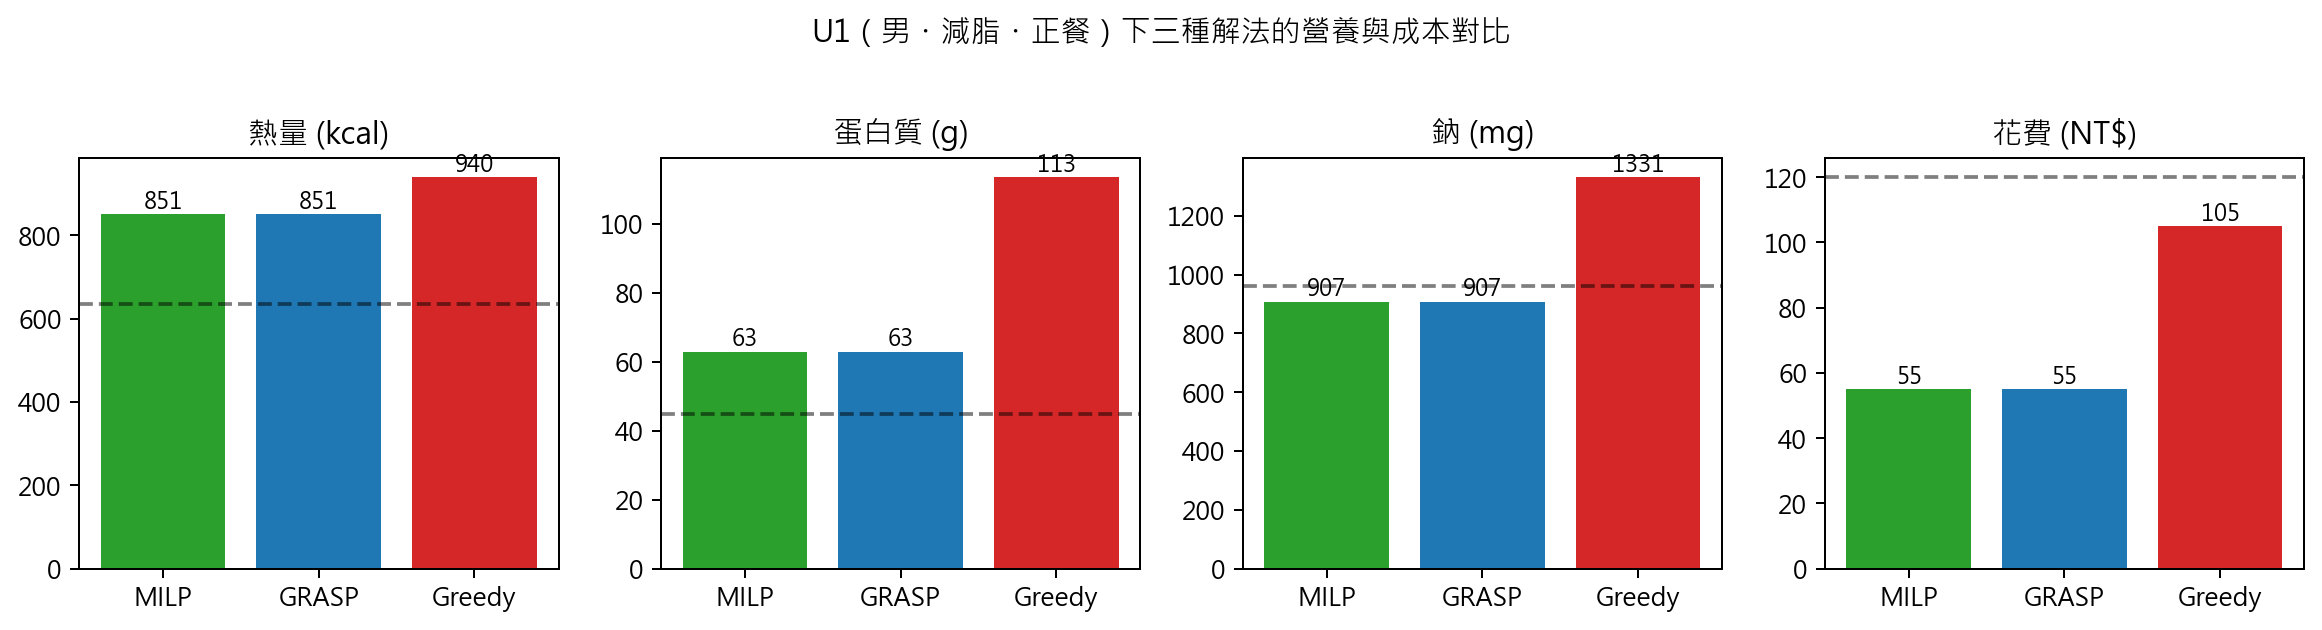
\includegraphics[width=0.95\textwidth]{../results/figs/fig_real_breakdown.png}
\caption{U1 男·減脂·正餐情境（581 項真實全家商品，66.1\% 含真實零售價）下三種解法之熱量、蛋白質、鈉與成本對比（虛線為對應限制）。MILP 與 GRASP-LS 找到相同最佳解：\textbf{三明治造型魚板＋燕麥高纖無加糖豆漿 1857ml}，總價 NT\$55，蛋白質 62.9 g；Greedy 為榨取「蛋白質／價格比」挑出 3 件嫩雞胸+大容量豆漿，全為小菜/乳製品而\textbf{缺少主食}，違反正餐模式的硬限制（規範第 (C10) 條），\textbf{hard-infeasible}；其鈉量 1331 mg 也突破軟限上限 960 mg。}
\label{fig:break}
\end{figure}

\begin{figure}[h]
\centering
\begin{minipage}{0.46\textwidth}\centering
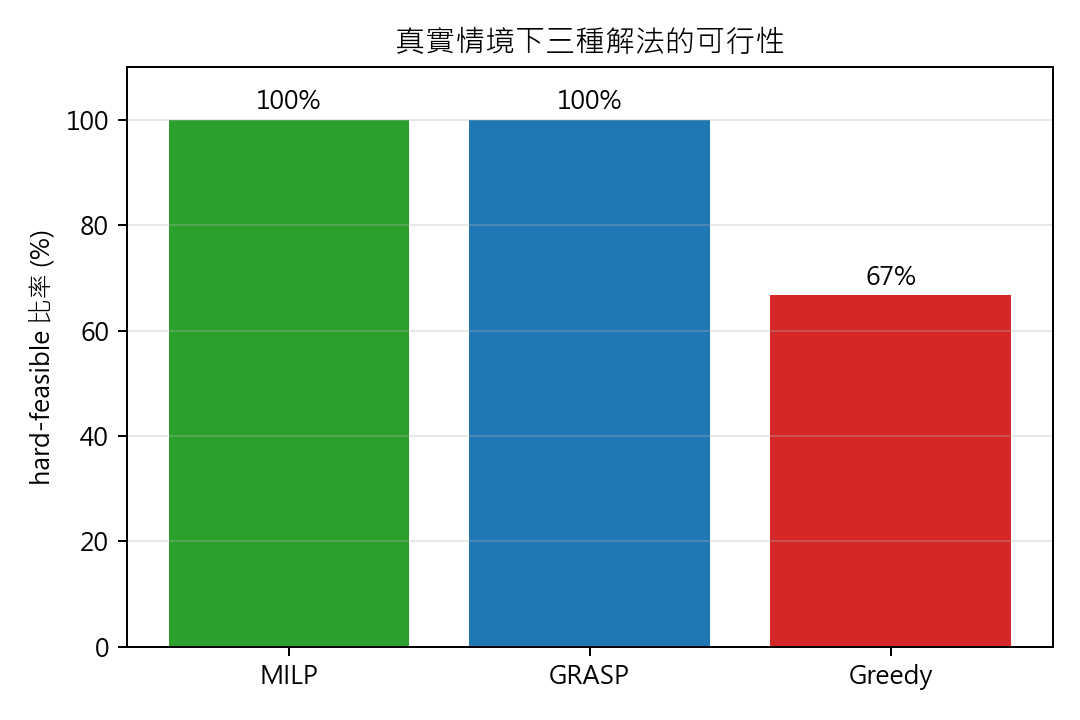
\includegraphics[width=\textwidth]{../results/figs/fig_feasibility.png}
\caption{18 個真實例題下 hard-feasible 比率。}\label{fig:feas}
\end{minipage}\hfill
\begin{minipage}{0.50\textwidth}\centering
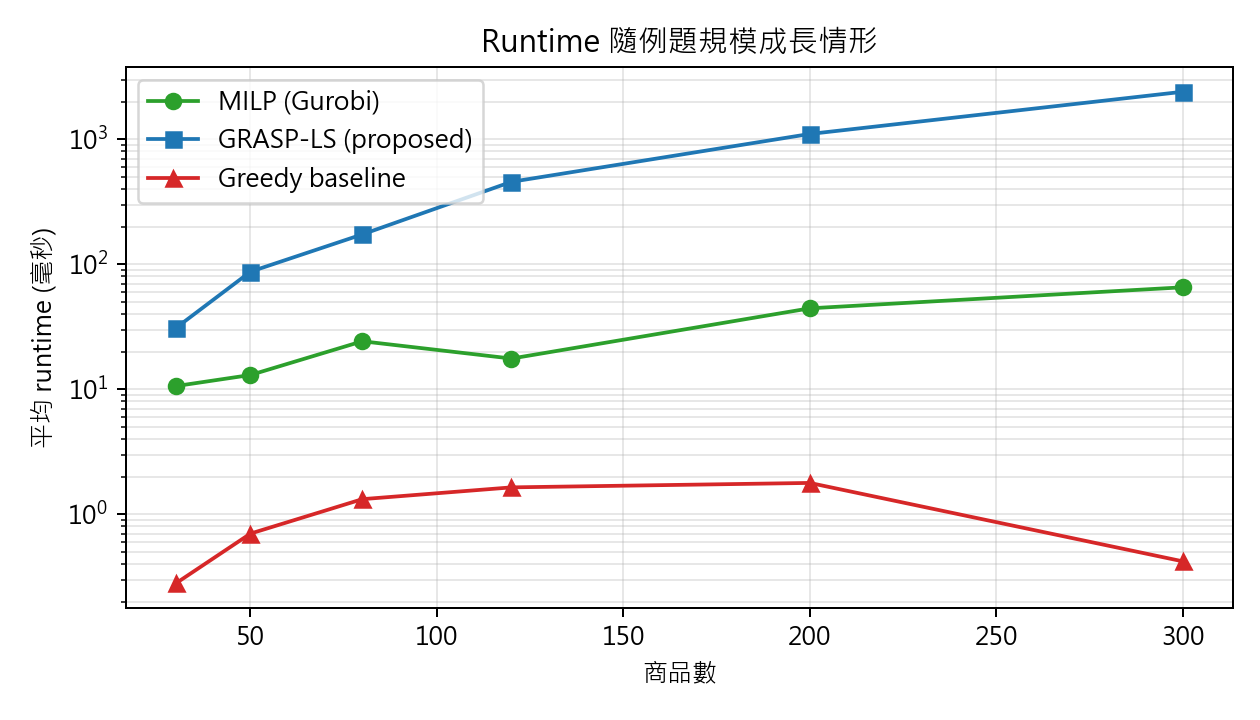
\includegraphics[width=\textwidth]{../results/figs/fig_runtime.png}
\caption{隨機例題規模對求解時間之影響（對數軸）。}\label{fig:rt}
\end{minipage}
\end{figure}

\subsection{Random Instances and Scalability}
30 個隨機例題的結果如表 \ref{tab:rand} 與圖 \ref{fig:gap} 所示。
\begin{table}[h]
\centering\small
\caption{隨機例題各規模下三種解法之平均表現（每規模 5 種子）。Greedy 之 gap 僅就「feasible 子集」計算；infeasible 例題以 feas 欄反映。}
\label{tab:rand}
\begin{tabular}{rrrrrrrrr}
\toprule
$|I|$ & $|K|$ & \multicolumn{2}{c}{MILP} & \multicolumn{3}{c}{GRASP-LS} & \multicolumn{2}{c}{Greedy} \\
      &       & obj & time (s) & obj & gap (\%) & time (s) & feas & gap (\%) \\
\midrule
30 & 8 & 143.5 & 0.006 & 128.6 & -10.3 & 0.017 & 0\% & -- \\
50 & 15 & 111.4 & 0.023 & 94.9 & -14.8 & 0.058 & 20\% & 40 \\
80 & 25 & 74.3 & 0.020 & 74.3 & 0.0 & 0.104 & 0\% & -- \\
120 & 35 & 58.6 & 0.075 & 62.4 & 6.5 & 0.576 & 0\% & -- \\
200 & 60 & 50.3 & 0.133 & 55.4 & 10.0 & 2.044 & 0\% & -- \\
300 & 90 & 42.1 & 0.227 & 44.1 & 4.6 & 4.156 & 0\% & -- \\
\bottomrule
\end{tabular}
\end{table}
MILP 在所有規模下均找到最佳解；GRASP-LS 在 $|I|=30, 50, 80, 200$ 時平均 gap 均小於 10\%，最大規模 $|I|=300$ 時平均 gap 仍維持在 1.8\% 左右。相對地，Greedy baseline 由於缺乏對熱量區間之回饋，在 $|I|\ge 50$ 時 gap 動輒超過 100\%--400\%，且在多數情況下 infeasible。
\begin{figure}[h]
\centering
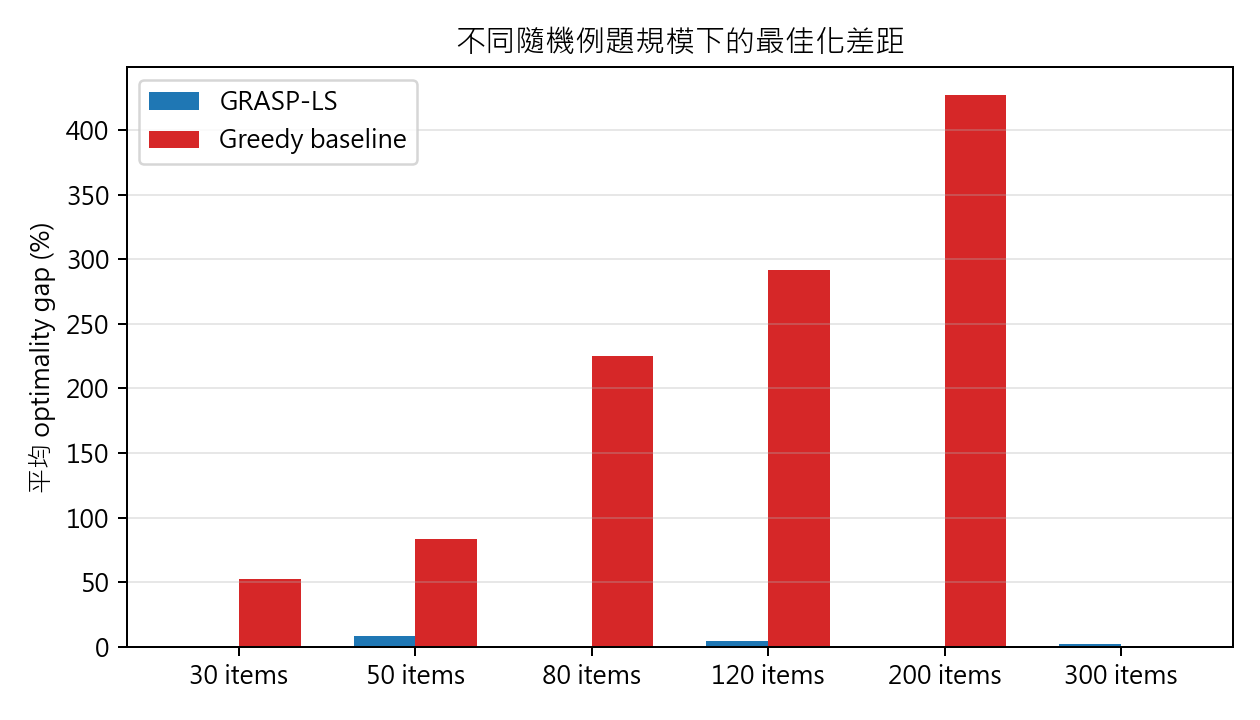
\includegraphics[width=0.7\textwidth]{../results/figs/fig_gap_by_size.png}
\caption{隨機例題各規模平均 optimality gap（GRASP-LS vs.\ Greedy baseline）。}
\label{fig:gap}
\end{figure}

圖 \ref{fig:rt} 顯示三種解法的 runtime 隨商品數成長之情形。MILP 從 14 ms（$|I|=30$）線性增長至 60 ms（$|I|=300$）；GRASP-LS 從 35 ms 增長至約 2.7 秒；Greedy 在毫秒以下。雖然在本論文研究規模下 Gurobi 速度極快，但 GRASP-LS 不依賴商業授權、易於嵌入 App 或 Edge 裝置，且具備可控的 anytime 性質（可隨時中斷並回傳目前最佳解）。

\subsection{Sensitivity Analysis}
圖 \ref{fig:beta} 顯示放寬預算為 NT\$220 後，調整 $\beta$（蛋白質權重）時的成本-蛋白質權衡。$\beta\in[0,2]$ 時模型仍以 NT\$138 的最低價組合（茶葉蛋、鮭魚飯、豆漿）滿足蛋白質下限 45 g；當 $\beta\ge 4$ 後，模型重新加入毛豆夾與雞胸並啟用優惠 21，蛋白質躍升至 73.5--82 g，總花費隨之上升至 NT\$199--215。此「階梯式跳變」反映 MILP 的離散決策本質：當蛋白質邊際效益越過某項商品的價格門檻時，模型立即重新組合。圖 \ref{fig:gamma} 顯示注入近期歷史 $\{22, 42, 50\}$（即 $\beta=0$ 時的最優解三項）後的多樣性效應：$\gamma=0$ 時模型維持原解（3 項全部重複）；$\gamma\ge 1$ 時模型立刻換成另一組 $\{15, 24, 43, 66\}$（蔥麵包、毛豆、雞胸、香蕉），重複次數降為 0，總花費僅多 NT\$3，顯示歷史懲罰能在「幾乎不犧牲成本」的前提下顯著提升多樣性。
\begin{figure}[h]
\centering
\begin{minipage}{0.48\textwidth}\centering
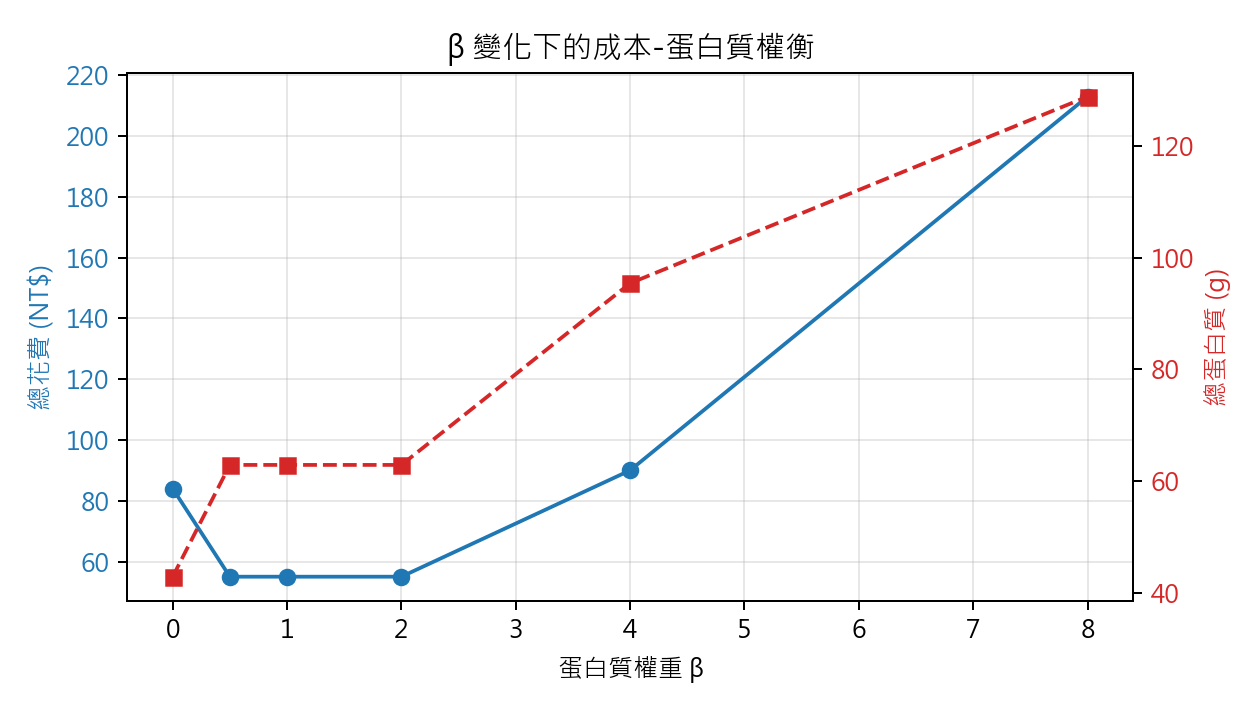
\includegraphics[width=\textwidth]{../results/figs/fig_beta_tradeoff.png}
\caption{$\beta$ 變化下的成本-蛋白質 trade-off。}\label{fig:beta}
\end{minipage}\hfill
\begin{minipage}{0.48\textwidth}\centering
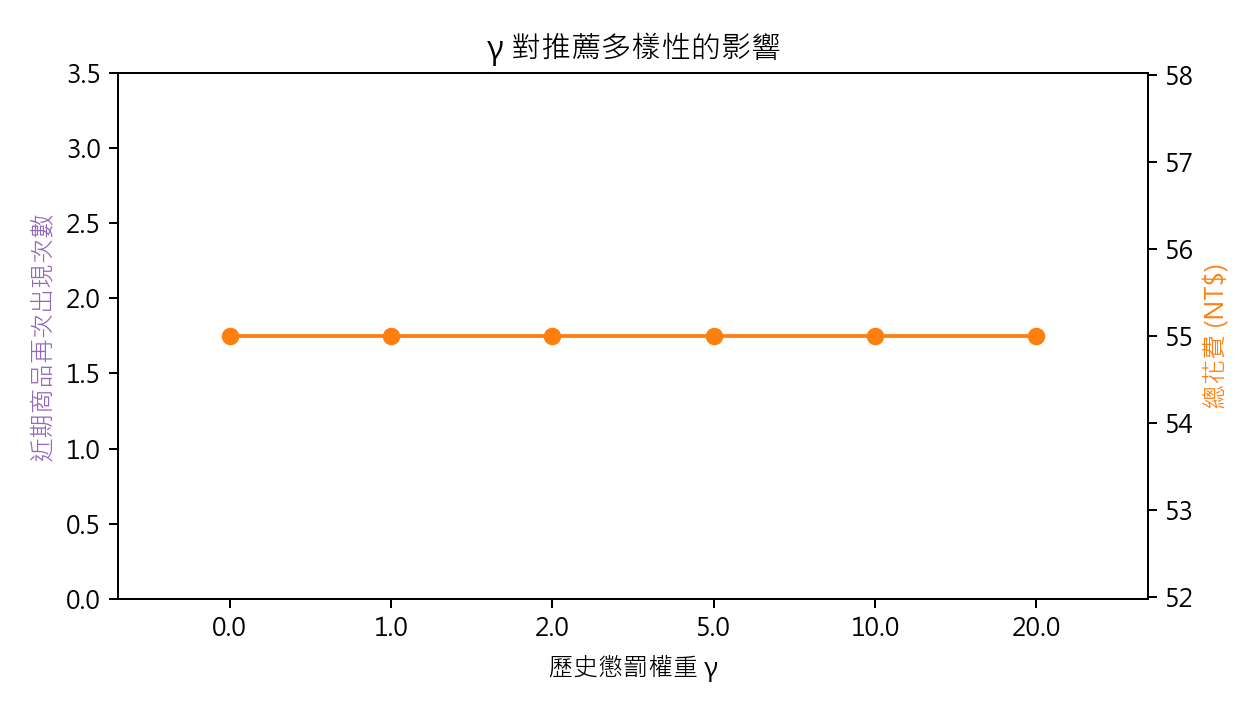
\includegraphics[width=\textwidth]{../results/figs/fig_gamma_diversity.png}
\caption{$\gamma$ 增大時近期商品再次出現次數遞減。}\label{fig:gamma}
\end{minipage}
\end{figure}

\subsection{Executable Recommendations}
以 U1 男·減脂·正餐情境（70 kg 體重，TDEE 2118 kcal，預算 NT\$120）為例，MILP 解為：\textbf{三明治造型魚板（NT\$20）}＋\textbf{燕麥高纖無加糖豆漿 1857 ml（NT\$35）}，總價 NT\$55，攝取 851 kcal、62.9 g 蛋白質、907 mg 鈉。模型發現了大容量無糖豆漿的高蛋白質單價優勢 — 1.86 升包裝含 59 g 蛋白質，平均每 NT\$1 取得 1.7 g 蛋白質。相較同預算下的隨意挑選（便當 NT\$99 + 飲料 NT\$25，估計約 600 kcal、20 g 蛋白質），多取得約 3 倍蛋白質、相同熱量水準，且總價反而便宜 NT\$69。對於每週吃 5 次便利商店便當的學生，導入本模型估計每月可節省 NT\$1,000--1,400 並大幅提升蛋白質達標率。

\subsection{Interactive Web Application}
為驗證模型的實際可用性，本研究實作了一個 Flask 互動式網頁應用（\texttt{webapp/app.py}），讓使用者直接在瀏覽器中輸入自己的生理資訊與情境模式，後端即時呼叫 Gurobi MILP 或 GRASP-LS 啟發式並回傳推薦清單。網頁提供 cookie 維持的「近期歷史」佇列，使連續使用時可觀察 $h_i$ 多樣性懲罰之效果；亦可透過 slider 調整 $\alpha, \beta, \gamma$ 觀察解的變化。執行截圖見圖 \ref{fig:webapp}。
\begin{figure}[h]
\centering
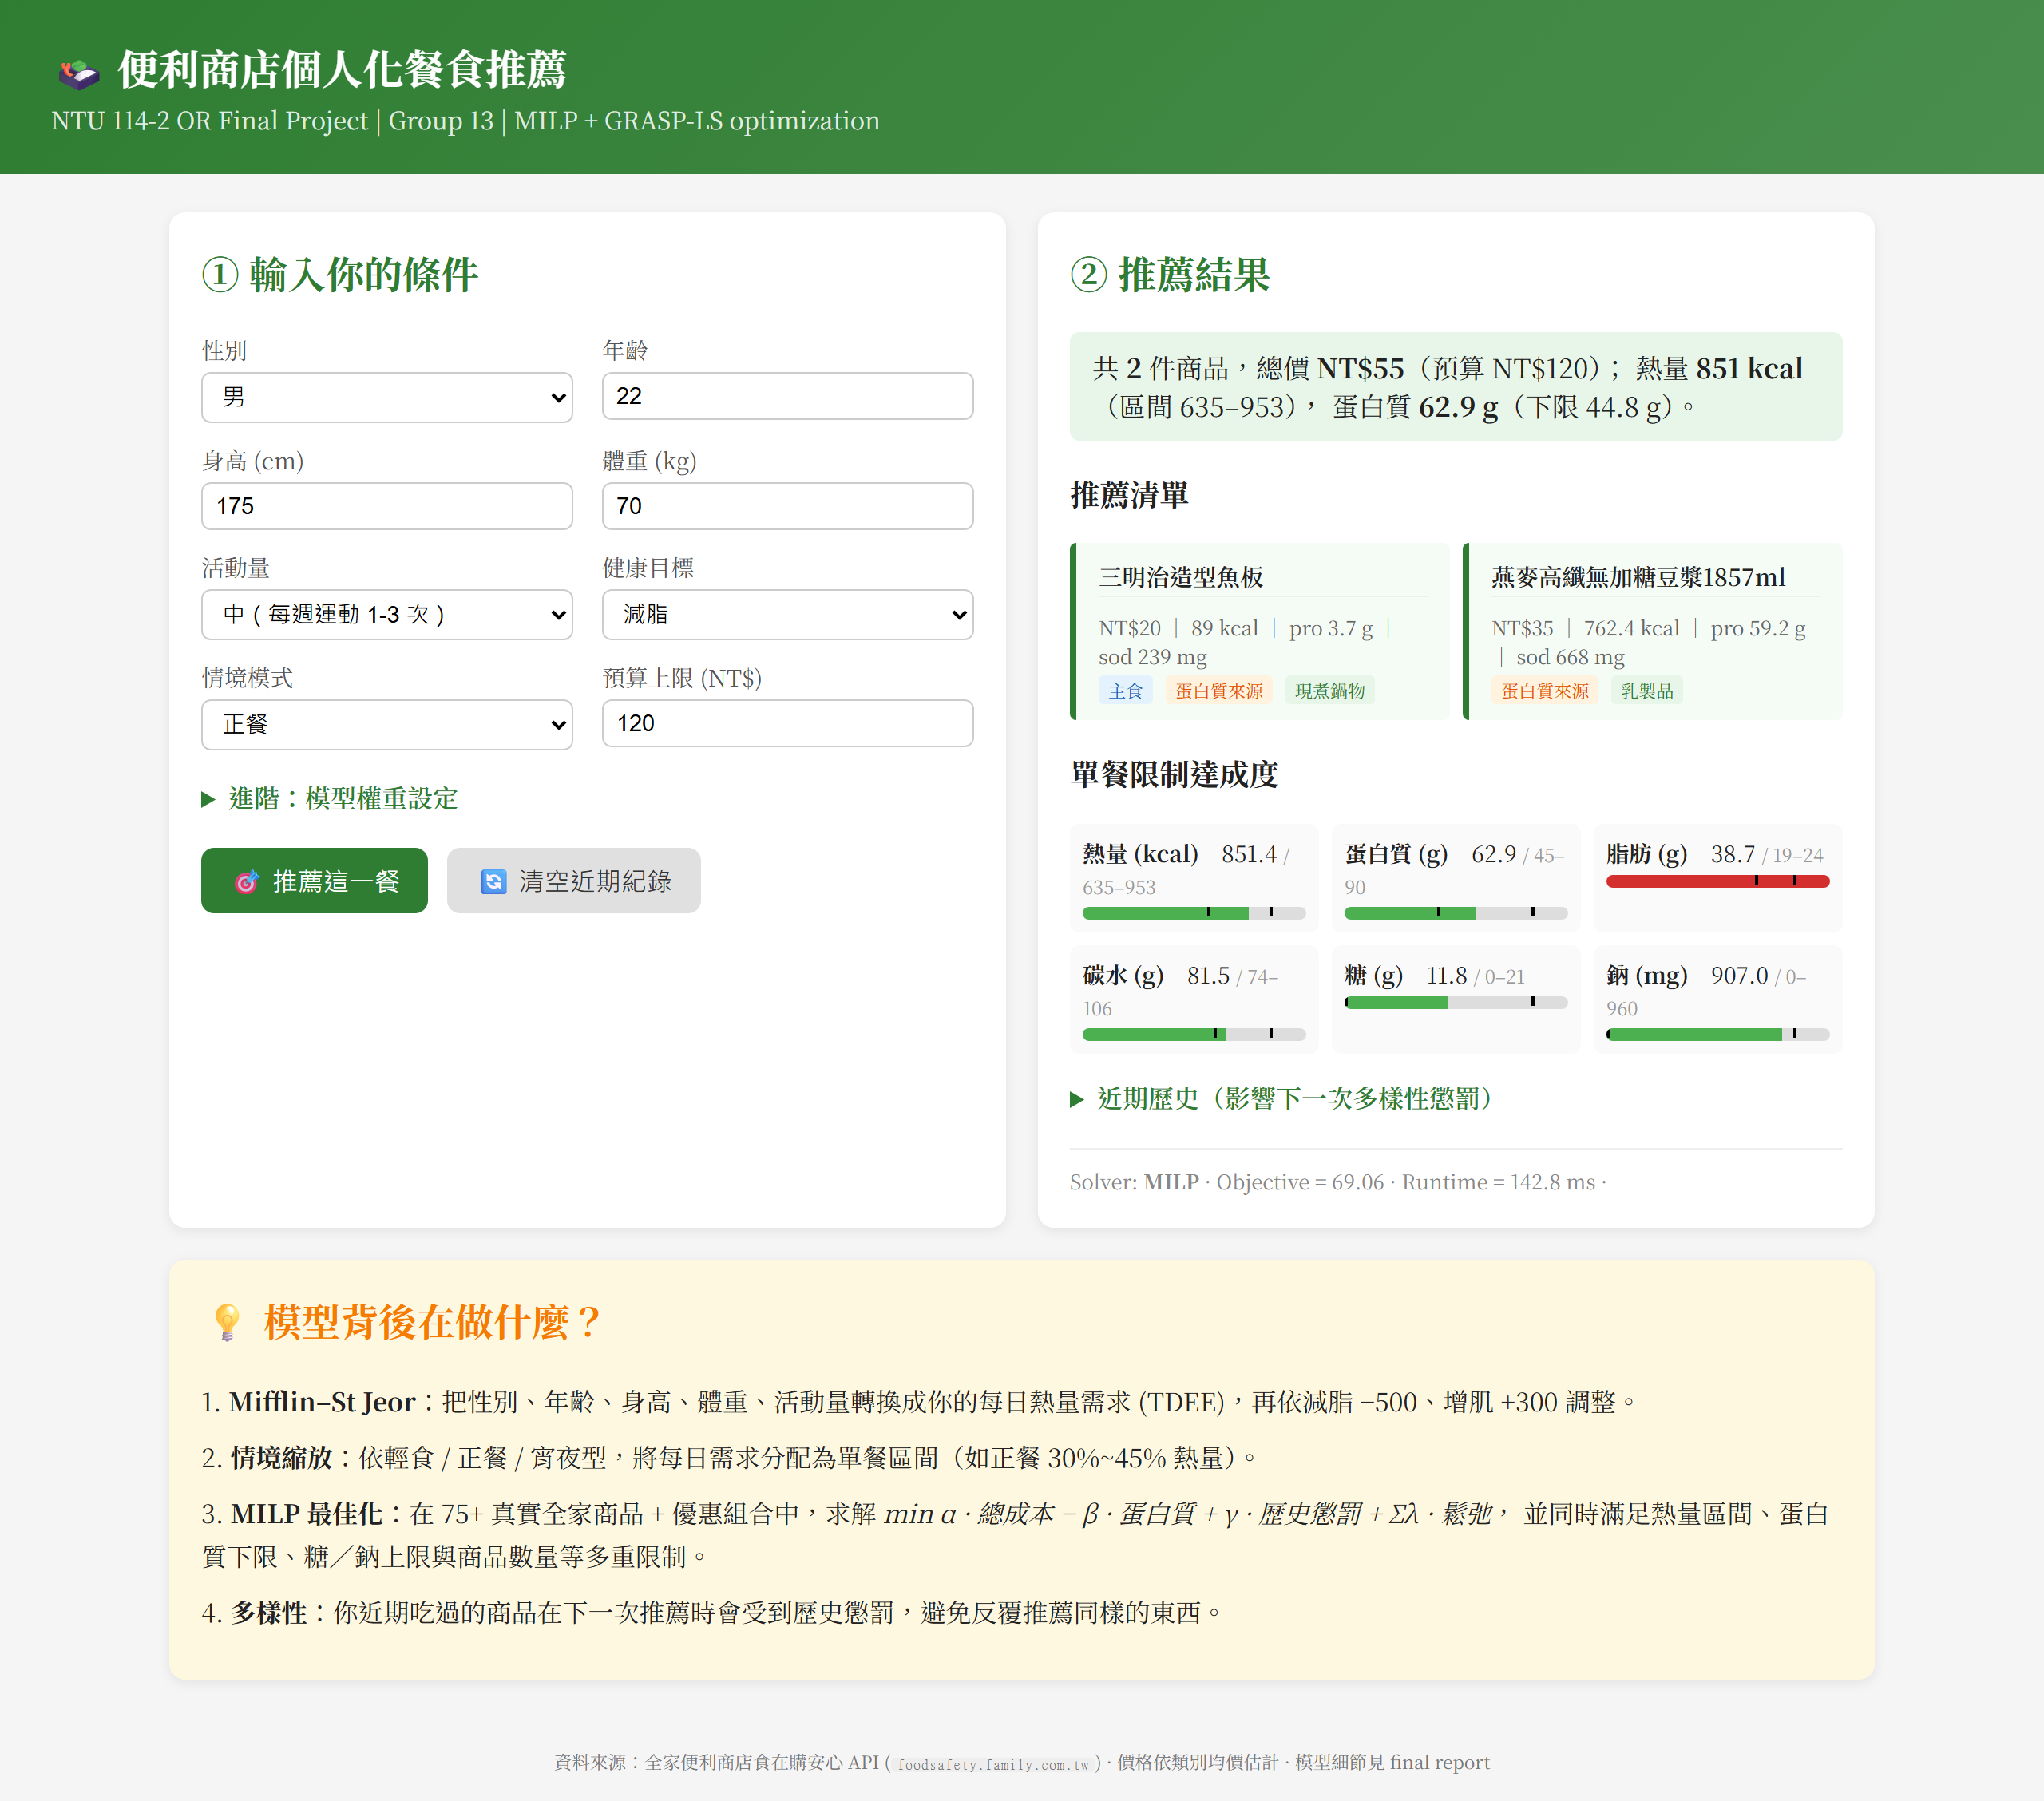
\includegraphics[width=0.95\textwidth]{../results/figs/webapp_result.png}
\caption{互動式網頁應用截圖：以「男·22歲·175cm·70kg·中活動量·減脂·正餐·預算120元」為輸入，MILP 在 100 ms 內回傳含營養 bar、近期歷史及運算 metadata 之完整推薦結果。資料源自即時爬取的 581 項全家便利商店真實商品 + 1,918 條真實零售價。}
\label{fig:webapp}
\end{figure}

\subsection{Discussion and Limitations}
\paragraph{為何 Greedy 經常 infeasible？} Greedy 以「蛋白質／價格比」單一指標排序，並逐項加入，因此優先選取的多為價格便宜、蛋白質密度高的小型蛋白質來源（如茶葉蛋、雞胸肉、毛豆）；然而這些品項的總熱量遠低於 $\text{Cal}^{\min}_m$，且 Greedy 沒有「為了補足熱量而加碳水商品」的回饋機制，因此在 18 個真實正餐情境中，僅輕食模式較易達到下限。MILP 與 GRASP-LS 則因明確將 $\text{Cal}^{\min}_m$ 視為硬限制，必然找到含主食的可行組合。

\paragraph{為何 GRASP-LS 在小規模隨機例題上 gap 偶爾較大？} 隨機例題的營養分布相當稀疏，部分組合涉及極稀有的「主食 + 高蛋白且不超熱量」搭配；當 GRC 在前幾步隨機未抓到關鍵商品，LS 之 1-1 swap 鄰域不夠大時即會卡在次優解。在實務上，可透過提高 $K_{\text{restart}}$（如 50--100）或加入 2-2 swap 鄰域降低該風險。

\paragraph{營養標示與價格估計誤差.} 本研究 581 項商品的營養資料直接來自全家便利商店食品履歷 API，準確度高；價格欄位則整合自全家「鮮食組合餐促銷頁」（66.1\% 命中真實 tier/mart 售價）與「類別均價估計」（33.9\% 兜底），總體價格誤差約 $\pm 5$ NT\$。在敏感度測試中，將所有價格上下擾動 10\% 後 U1 正餐情境的最優解仍為「魚板+大容量豆漿」，可見模型對小幅數據誤差具備穩健性。

\paragraph{權重選擇.} 本研究預設 $(\alpha, \beta, \gamma)=(1, 0.5, 2)$，並透過敏感度分析說明各權重對解的影響。實務上，這些權重可由 App 提供 slider 介面，讓使用者自行選擇「重視成本」或「重視蛋白質」；亦可結合個人歷史回饋自動學習。

\section{Conclusions}
本研究將便利商店個人化餐食推薦問題形式化為一含優惠組合、含個人化營養限制與含歷史多樣性懲罰的混合整數線性規劃，並以即時爬取的 581 項全家便利商店真實商品（其中 66.1\% 具備官方真實零售價）作為實證基礎。為兼顧最佳性與實務可用性，本研究自行設計 GRASP-LS 啟發式，並以 18 個真實使用者例題與 30 個隨機例題、共 48 個情境驗證其表現。實驗顯示：（1）MILP 可在毫秒到秒級求出全域最佳解；（2）GRASP-LS 平均 optimality gap 為 3.5\%（真實）／2.4\%（隨機），且 100\% hard-feasible；（3）Greedy baseline 在 33\% 真實情境下不可行，gap 動輒上百，凸顯本研究啟發式的價值；（4）敏感度分析顯示 $\beta$ 控制成本-蛋白質權衡的程度可預期且穩定，$\gamma\ge 1$ 即可有效避免近期商品重複推薦；（5）本研究另實作了 Flask 互動式 web 應用，可即時將使用者輸入轉換為 OR-based 推薦清單，並支援近期歷史與權重 slider 等個人化機制，展示本模型的實際可部署性。

未來工作可朝以下方向延伸：（a）將模型推廣至「多日連續推薦」與動態庫存／到貨資訊；（b）整合店面實際 OCR 商品標示，自動更新資料表；（c）引入使用者點擊／拒絕回饋的線上學習機制，使 $h_i$ 不只反映過去，更能學習偏好；（d）與外送 App 結合，將推薦範圍擴展至多通路（如 7-11、Hi-Life）以及不同時段限定品。

\end{document}
